\documentclass[a4paper]{article}
\usepackage{a4wide}
\usepackage{amsmath}
\usepackage{amsfonts}
  \DeclareMathOperator*{\argmax}{arg\,max}
  \newcommand{\ex}[1]{{\mathbb E}\left[ #1 \right]}
  \newcommand\norm[1]{\left\lVert#1\right\rVert}
\usepackage{booktabs}
\usepackage{csquotes}
\usepackage{upquote}
\usepackage{float}
\usepackage{graphicx}
\usepackage{enumerate}
\usepackage{subcaption}
\usepackage[most]{tcolorbox}
\usepackage{xcolor}
\usepackage{varwidth} 


\title{Pattern and Speech Recognition WS2015-16 \\ Exercise 9}
\author{Atanas Poibrenski(2554135), Marimuthu Kalimuthu(2557695), Furkat Kochkarov(2557017)}

\begin{document}
	\tcbset{
		enhanced,
		colback=red!5!white,
		boxrule=0.1pt,
		colframe=red!75!black,
		fonttitle=\bfseries
	}

\maketitle 
\begin{center}
	\textbf{Neural Networks}
\end{center}

\section*{Implementation of the NN}
\begin{itemize}
	\item See `predict.m'. It returns a vector of dimension 400x1
	\item See `trainNetwork.m'
	\item We use \textit{rand} function in matlab for initializing the parameters using uniform distribution.
	\item Done. We use \textit{randperm} in matlab for shuffling the data. 
	Plots of the errors for different learning rates are as follows:

	\begin{tcolorbox}
	\begin{figure}[H]
		\begin{center}
			\includegraphics[width=0.9\textwidth]{learningrate0001.eps}
			\caption{ Learning rate 0.001}\label{fig:learn0.001}
		\end{center}
	\end{figure}
	\end{tcolorbox}
	
	\begin{tcolorbox}
		\begin{figure}[H]
			\begin{center}
				\includegraphics[width=0.9\textwidth]{learningrate001.eps}
				\caption{ Learning rate 0.01}\label{fig:learn0.01}
			\end{center}
		\end{figure}
	\end{tcolorbox}
	
	\begin{tcolorbox}
		\begin{figure}[H]
			\begin{center}
				\includegraphics[width=0.9\textwidth]{learningrate01.eps}
				\caption{ Learning rate 0.1}\label{fig:learn0.1}
			\end{center}
		\end{figure}
	\end{tcolorbox}
	
	\begin{tcolorbox}
		\begin{figure}[H]
			\begin{center}
				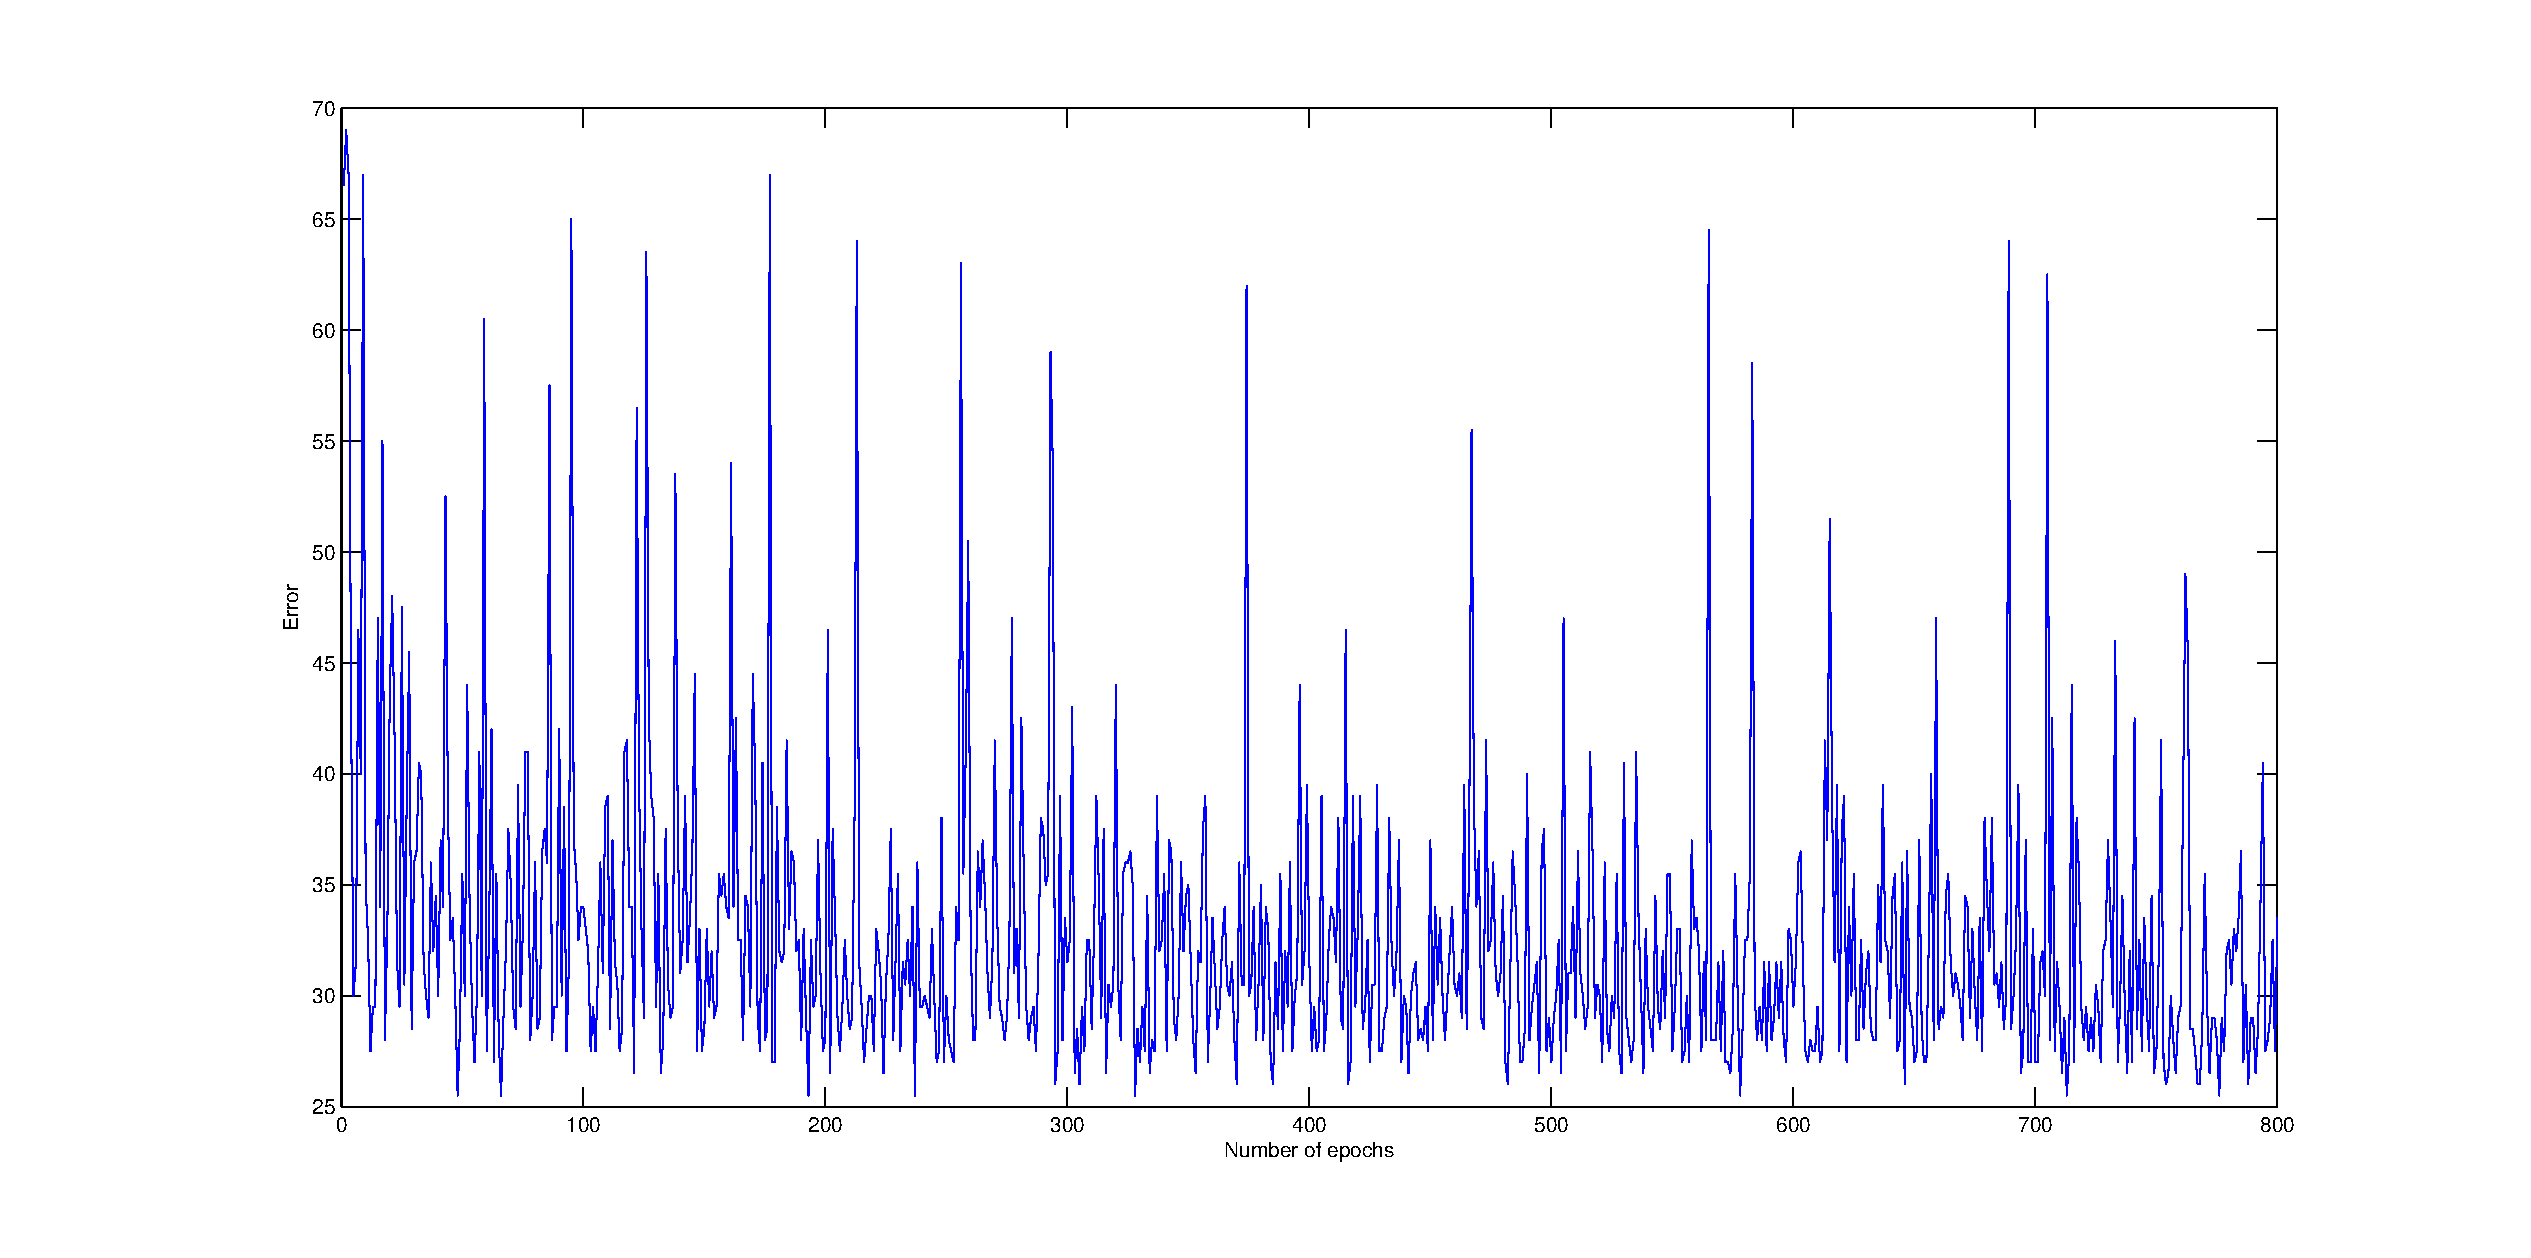
\includegraphics[width=1.0\textwidth]{learningrate1.eps}
				\caption{ Learning rate 1}\label{fig:learn1}
			\end{center}
		\end{figure}
	\end{tcolorbox}
	
	\textbf{Conclusions}: \newline
	  We choose to use the learning rate `0.1' because it converges faster than 0.001 \& 0.01 and is more stable than learning rate 1. (See Figure 1-4)
	  
	  In general, if the learning rate is high, the convergence is faster and it is slower when the learning rate is too low.

\end{itemize}

\section*{Plotting}
	\begin{itemize}
		\item See \textit{predict.m}
		\item See `plot\_boundary.m' for data \& decision boundary plot. \newline
		
		For 1 hidden neuron, we do not have a decision boundary because our network classifies every input as belonging to one class. So we cannot use the meshgrid and contour to plot. \newline
		
		The plots for the rest are as follows:
		
			\begin{tcolorbox}
				\begin{figure}[H]
					\begin{center}
						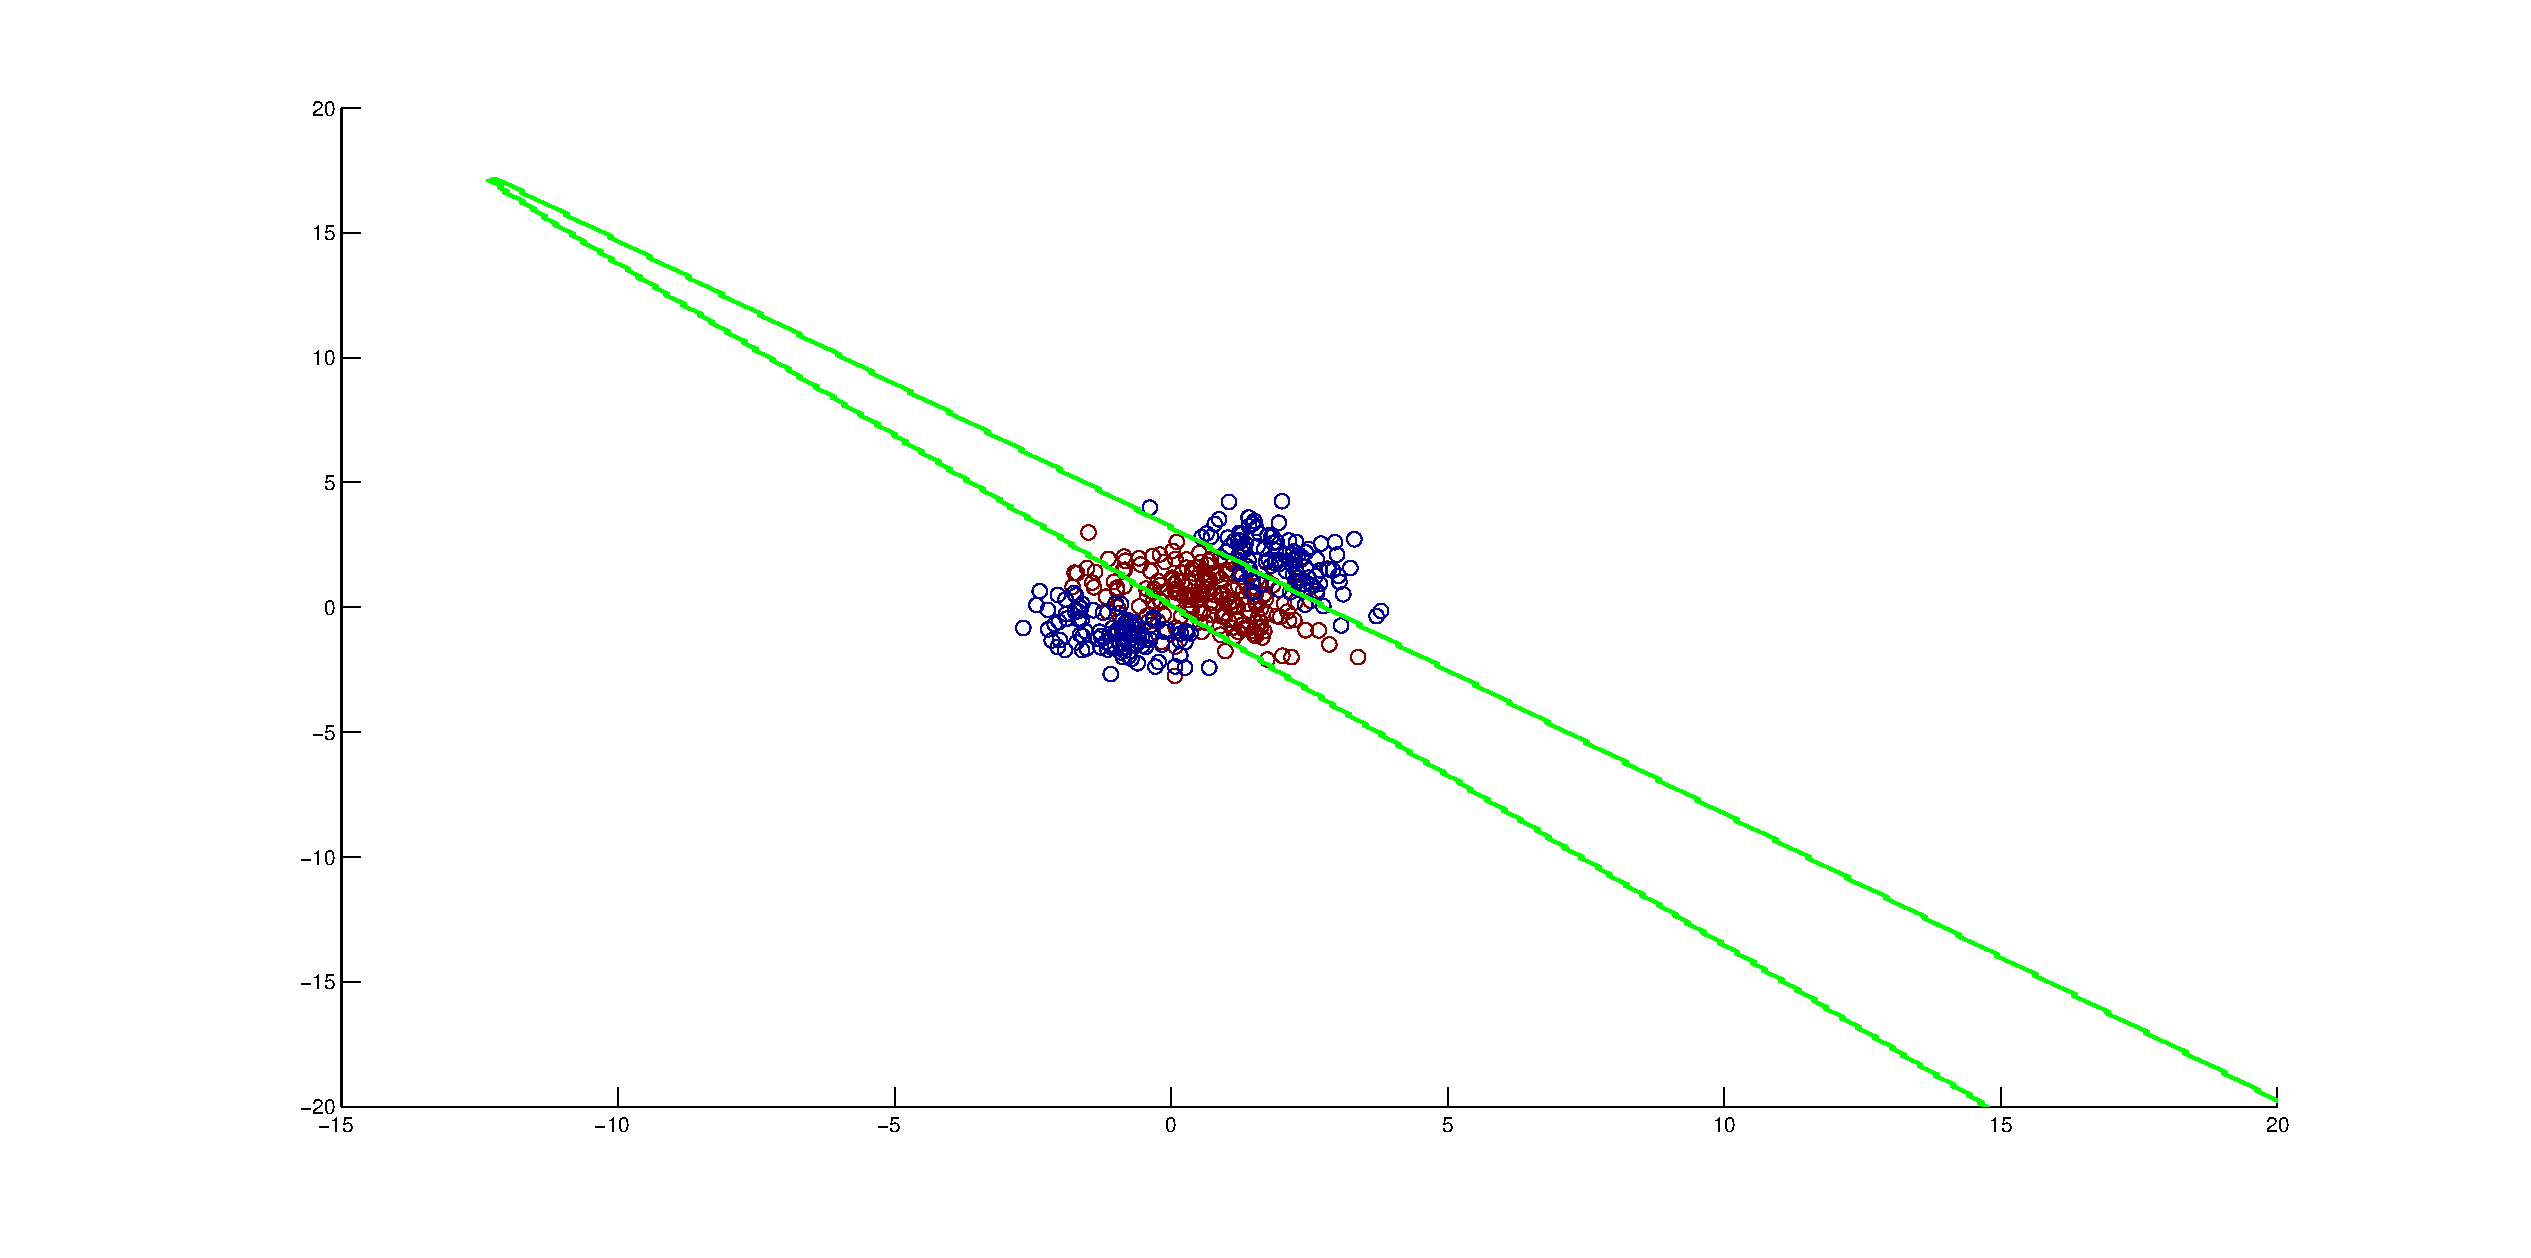
\includegraphics[width=0.9\textwidth]{decisionboundary2.eps}
						\caption{ Decision boundary for 2 hidden Neurons }\label{fig:decisionbound-2}
					\end{center}
				\end{figure}
			\end{tcolorbox}
			
			\begin{tcolorbox}
				\begin{figure}[H]
					\begin{center}
						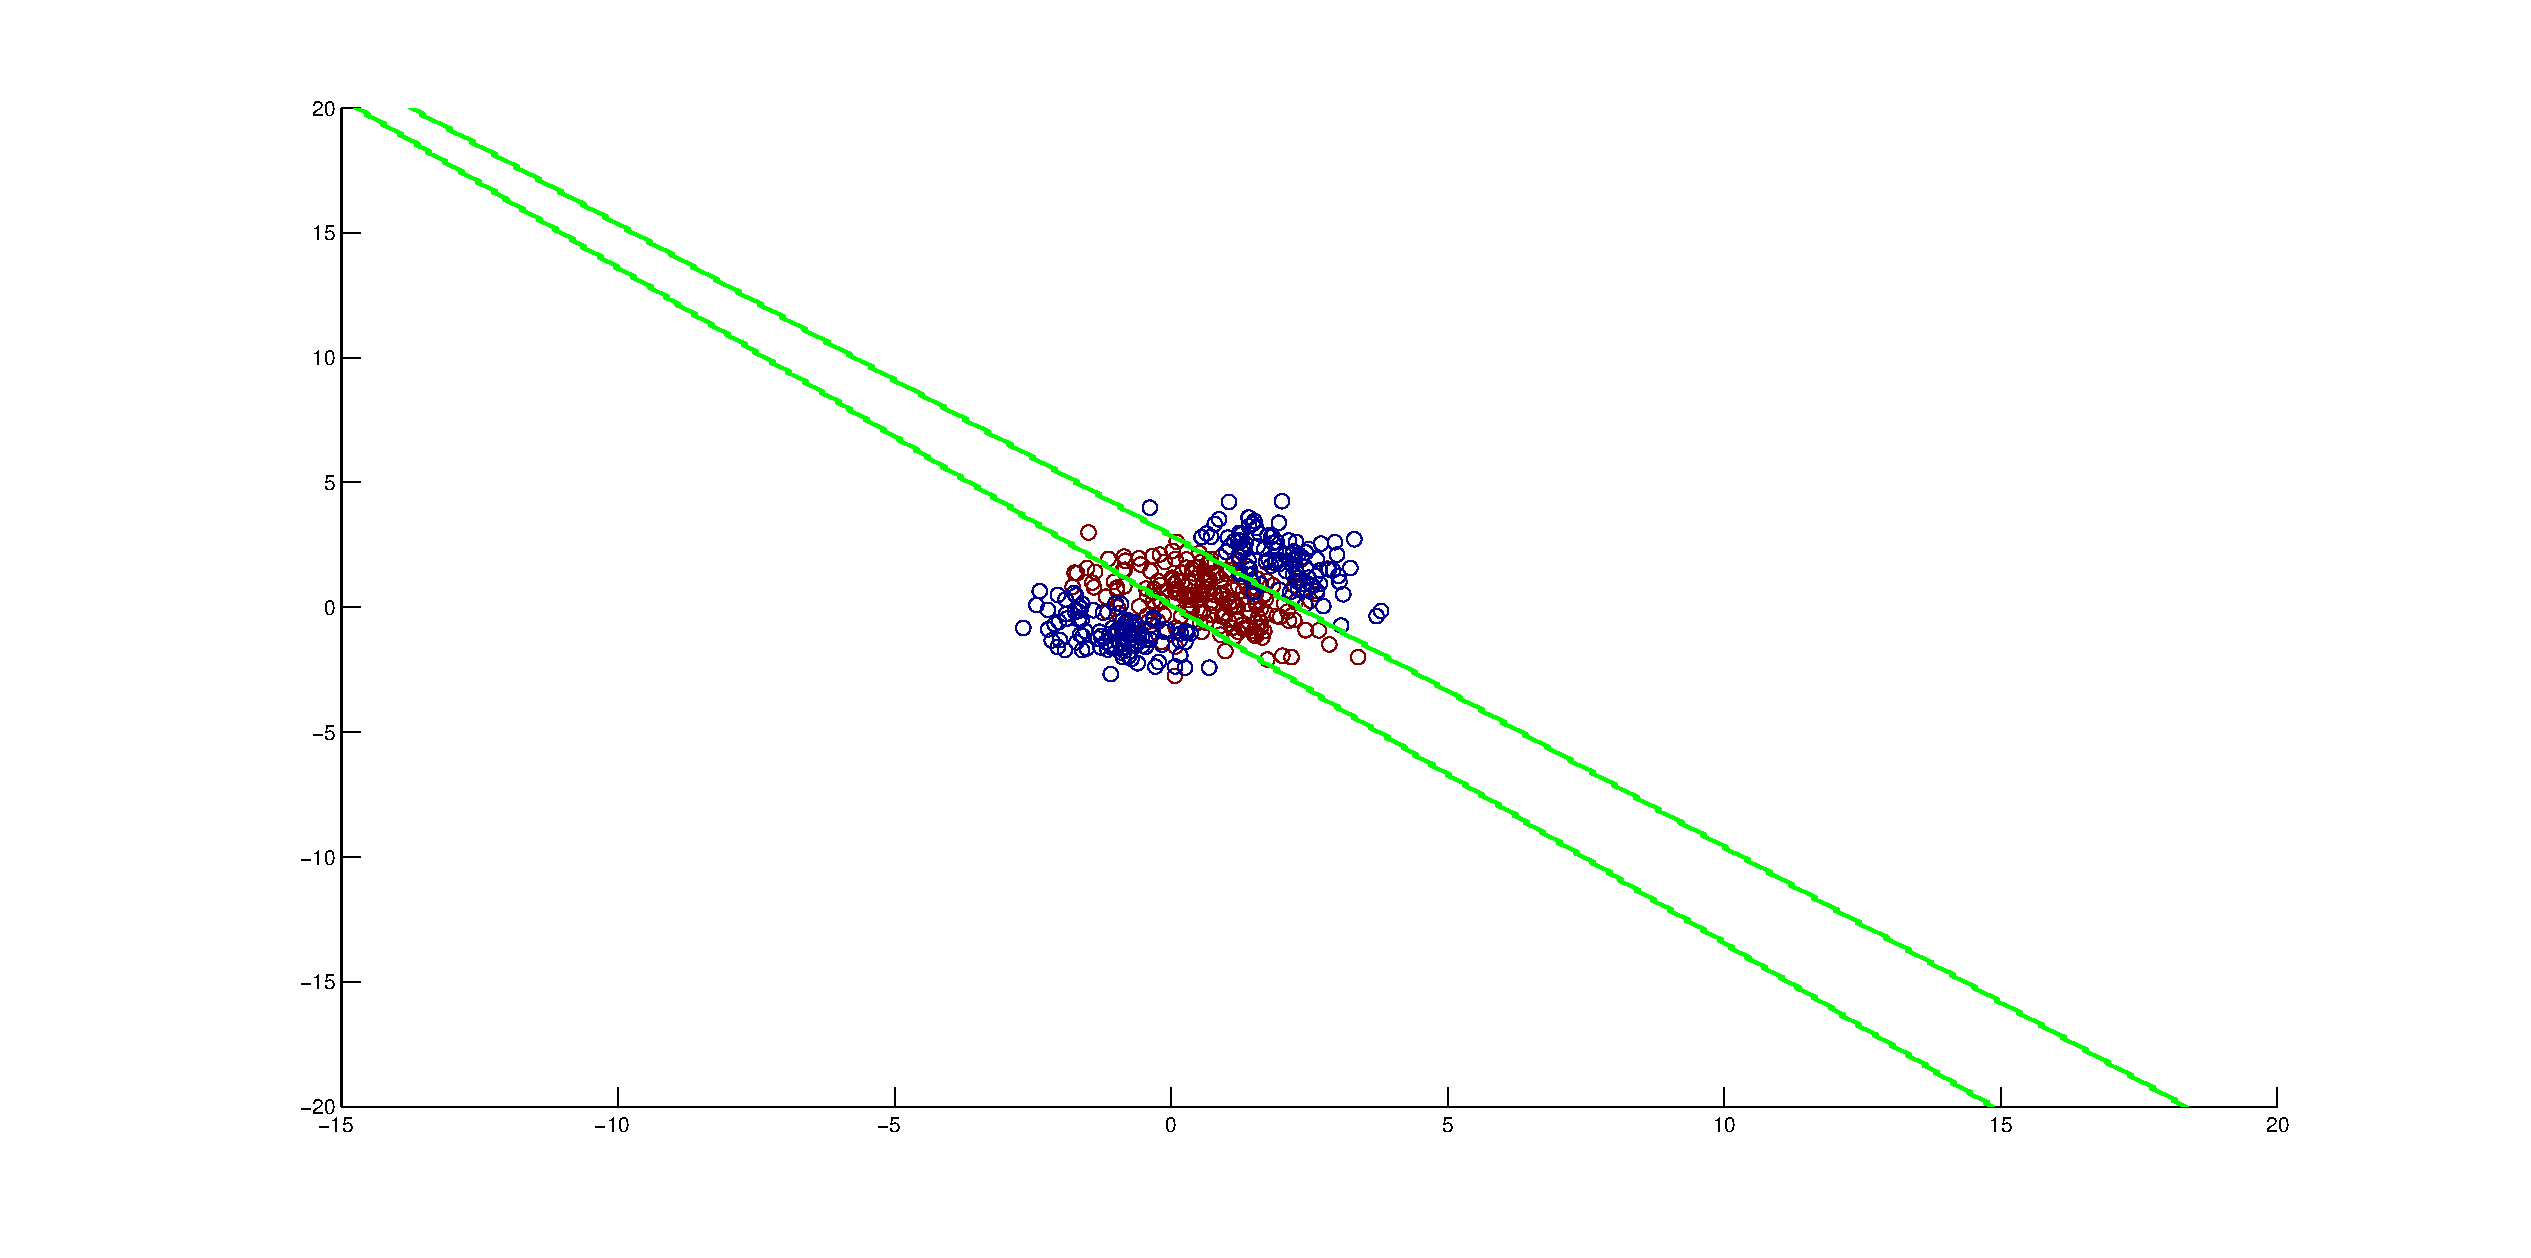
\includegraphics[width=0.9\textwidth]{decisionboundary3.eps}
						\caption{ Decision boundary for 3 hidden Neurons }\label{fig:decisionbound-3}
					\end{center}
				\end{figure}
			\end{tcolorbox}
			
			\begin{tcolorbox}
				\begin{figure}[H]
					\begin{center}
						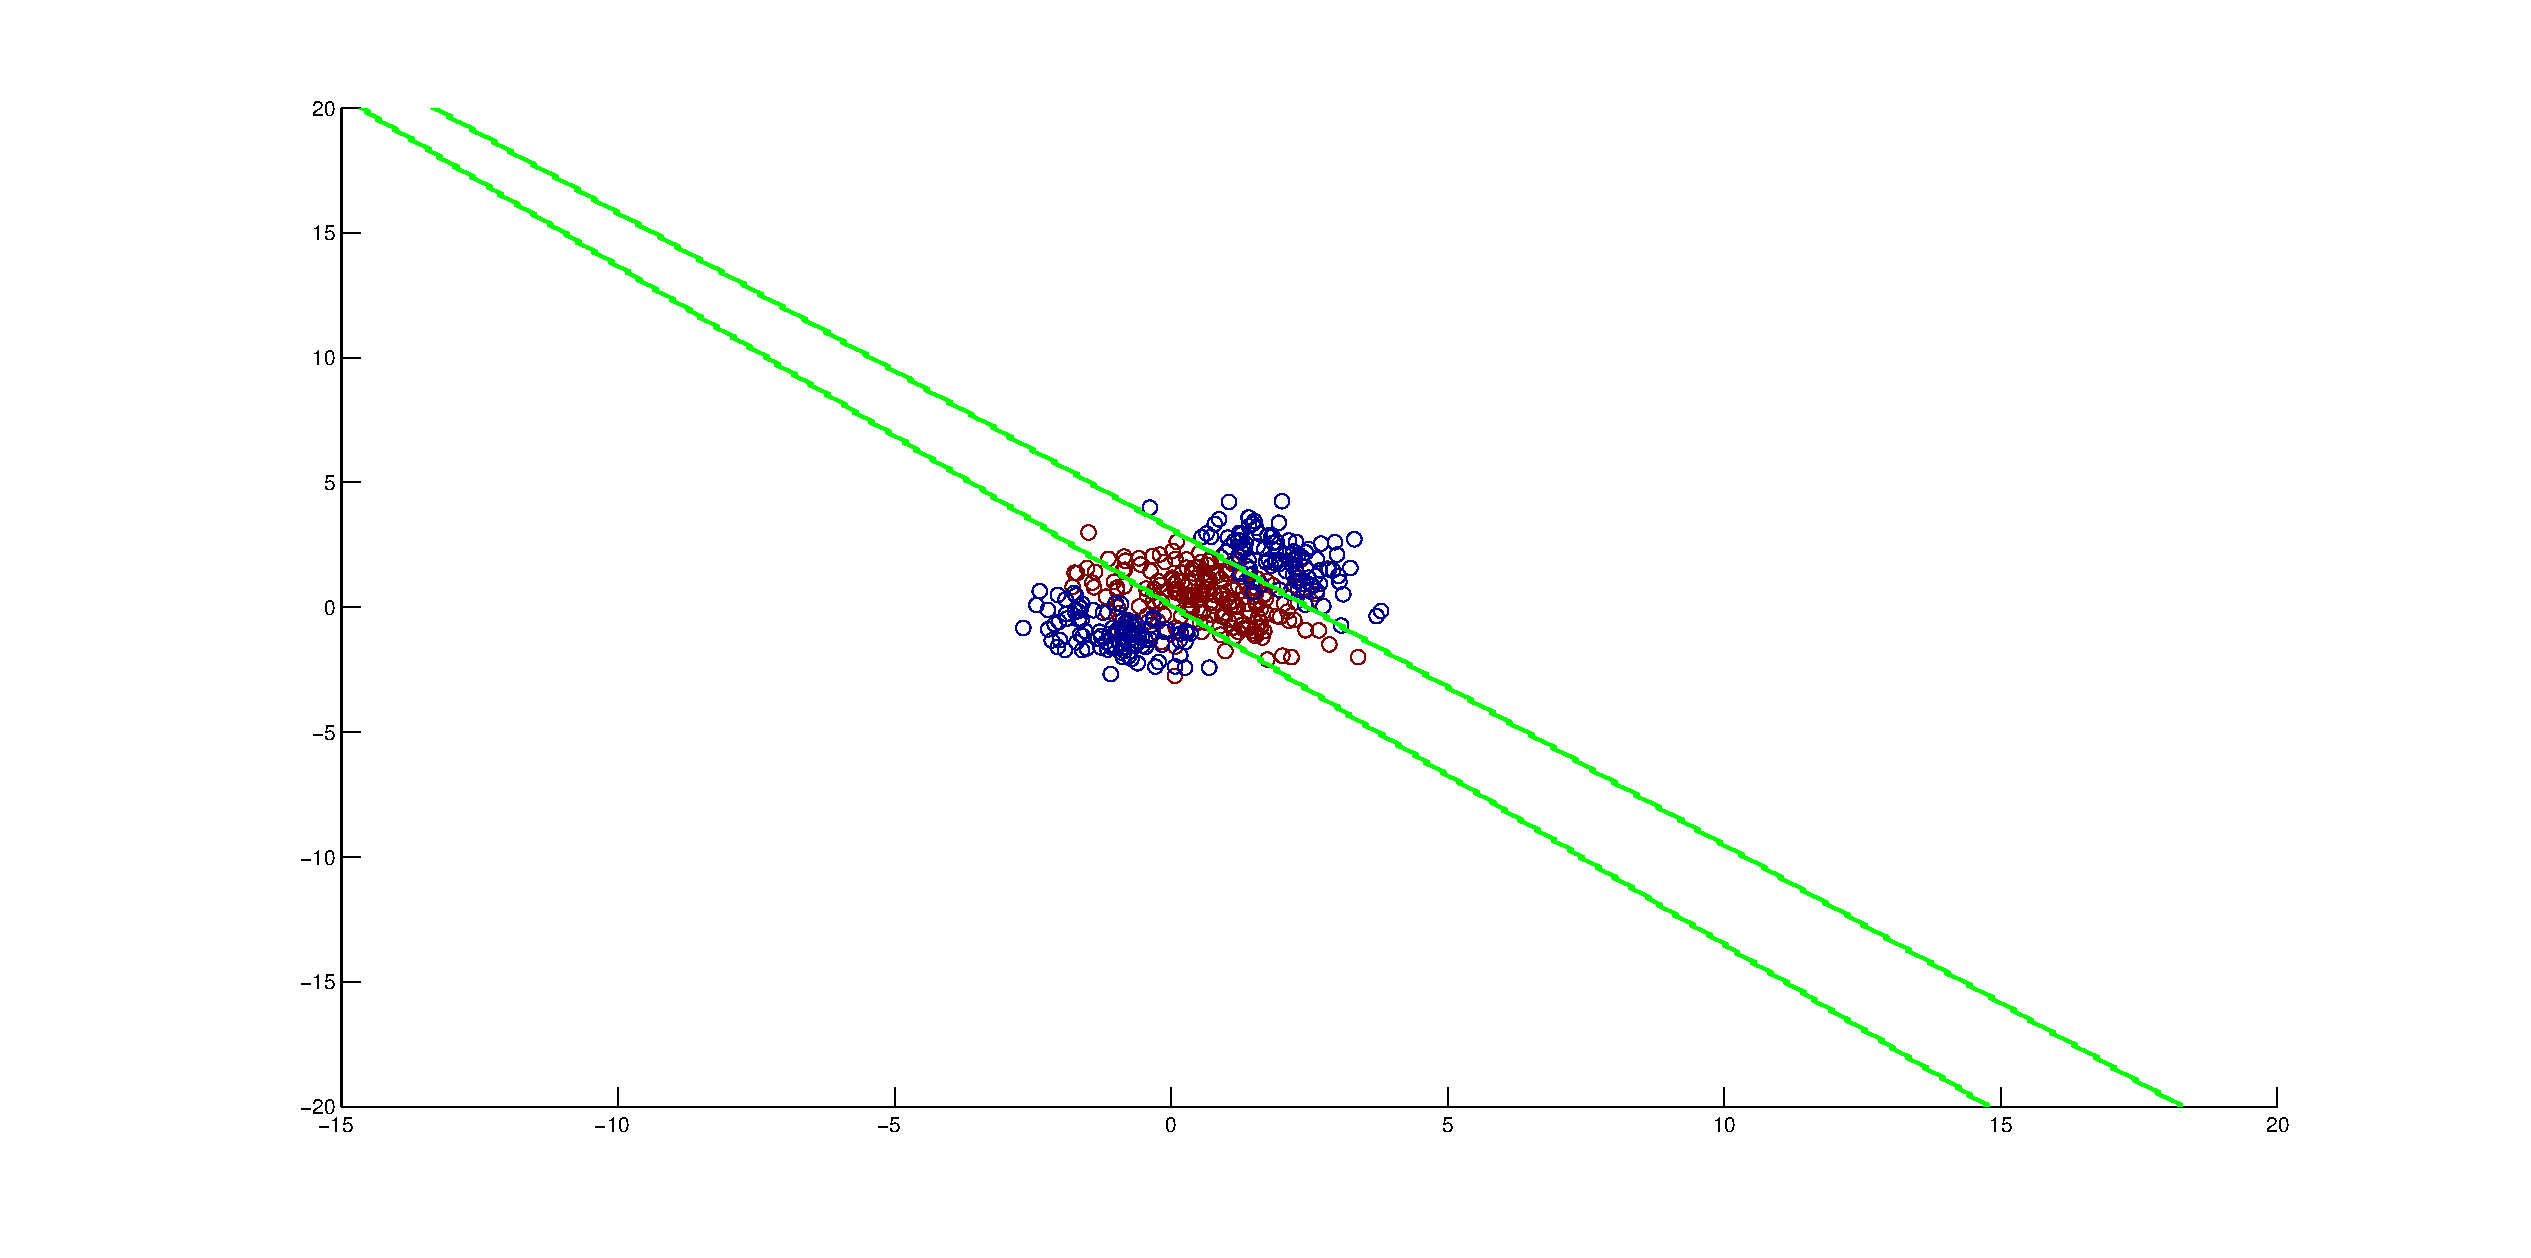
\includegraphics[width=0.9\textwidth]{decisionboundary4.eps}
						\caption{ Decision boundary for 4 hidden Neurons }\label{fig:decisionbound-4}
					\end{center}
				\end{figure}
			\end{tcolorbox}

			\begin{tcolorbox}
				\begin{figure}[H]
					\begin{center}
						\includegraphics[width=0.9\textwidth]{decisionboundary5.eps}
						\caption{ Decision boundary for 5 hidden Neurons }\label{fig:decisionbound-5}
					\end{center}
				\end{figure}
			\end{tcolorbox}					

			\begin{tcolorbox}
				\begin{figure}[H]
					\begin{center}
						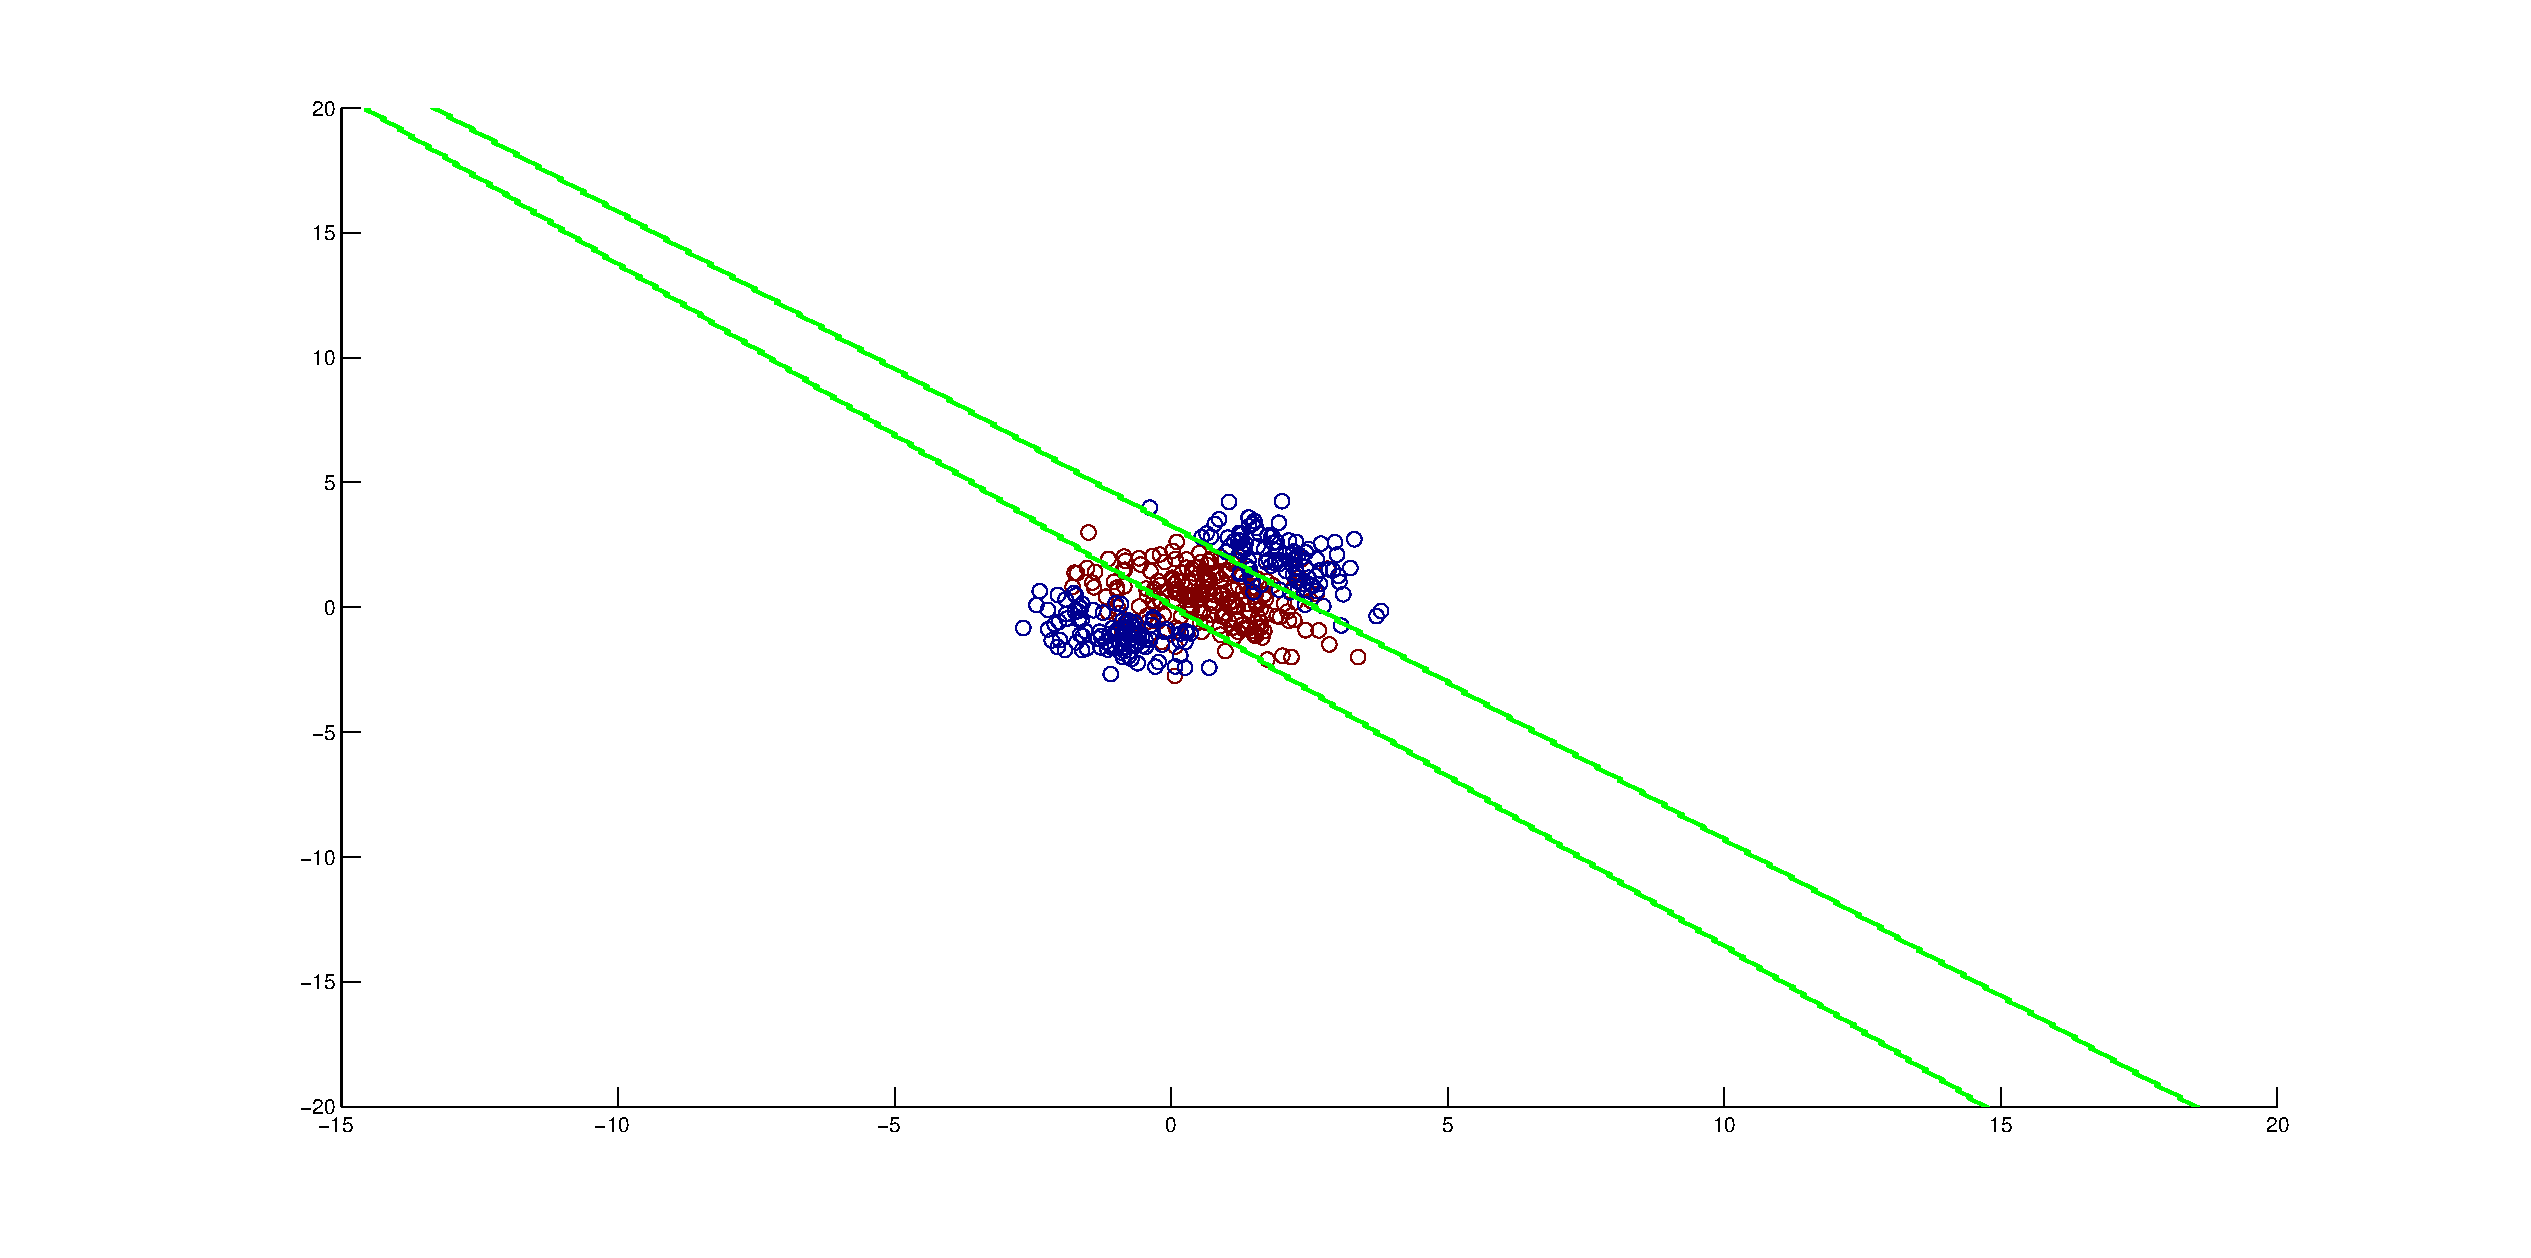
\includegraphics[width=0.9\textwidth]{decisionboundary6.eps}
						\caption{ Decision boundary for 6 hidden Neurons }\label{fig:decisionbound-6}
					\end{center}
				\end{figure}
			\end{tcolorbox}
						    
	\end{itemize}

\end{document}